% =============================================================================
% CAPÍTULO 2 - BLOQUE 2.1: FUNDAMENTOS MATEMÁTICOS DE LOS EMBEDDINGS,
% ESPACIOS LATENTES CONTINUOS Y SUPERACIÓN DEL PARADIGMA OCR
% =============================================================================

\subsection{Fundamentos Matemáticos de los Embeddings Multimodales y Espacios Semánticos Continuos}
\label{subsec:fundamentos_embeddings}

\subsubsection{El Problema del Análisis Secuencial y la Representación de Datos No Estructurados}
\label{subsubsec:problema_analisis_secuencial}

El crecimiento sostenido de los repositorios multimedia en entornos académicos, industriales y de radiodifusión ha puesto de manifiesto un problema metodológico fundamental en la ingeniería de datos: la extrema ineficiencia del análisis secuencial humano frente a volúmenes masivos de información no estructurada \cite{prajwal2025multimodal}. Históricamente, la tarea de localizar un evento singular dentro de un archivo de vídeo de larga duración (disciplina denominada en la literatura científica como \textit{Long-form Video Understanding} o \textit{Video RAG}) exigía bien un visionado manual exhaustivo por parte de operadores humanos, o bien una dependencia absoluta de metadatos descriptivos y etiquetas manuales generadas previamente a la indexación \cite{multi_rag2025}. En escenarios reales que abarcan desde archivos históricos de televisión y auditorías de videovigilancia hasta repositorios de clases universitarias grabadas o historiales médicos complejos, el etiquetado manual resulta técnica y económicamente inviable.

Para superar la barrera del procesamiento manual, los sistemas de Recuperación de Información (\textit{Information Retrieval}) evolucionaron hacia el paradigma de la Recuperación Aumentada por Generación (RAG, por sus siglas en inglés) \cite{prajwal2025multimodal}. No obstante, mientras que las arquitecturas RAG de primera generación operaban exclusivamente sobre cadenas de texto plano, los flujos multimedia contemporáneos requieren procesar, alinear e interpretar simultáneamente señales heterogéneas compuestas por secuencias de fotogramas, pistas de audio y texto libre \cite{prajwal2025multimodal, multi_rag2025}.

La base matemática que permite a un sistema computacional operar sobre formatos tan dispares sin recurrir a reglas heurísticas manuales es el concepto de \textbf{representación vectorial densa} o \textbf{\textit{embedding}} \cite{gemini_emb2_docs}. Un \textit{embedding} es una proyección matemática que transforma un objeto de entrada arbitrario $x$ (ya sea una oración en lenguaje natural, una matriz de píxeles correspondiente a un fotograma de vídeo o una onda acústica) en un vector de números reales en coma flotante $\mathbf{v} \in \mathbb{R}^d$ dentro de un espacio métrico continuo de dimensión $d$, según se formaliza en la Ecuación~\eqref{eq:proyeccion_multimodal} \cite{gemini_emb2_docs}:

\begin{equation}
f_{\theta}: \mathcal{X}_{\text{texto}} \cup \mathcal{X}_{\text{imagen}} \cup \mathcal{X}_{\text{vídeo}} \cup \mathcal{X}_{\text{audio}} \cup \mathcal{X}_{\text{PDF}} \longrightarrow \mathbb{R}^d
\label{eq:proyeccion_multimodal}
\end{equation}

donde $f_{\theta}$ representa una red neuronal profunda parametrizada por los pesos $\theta$ (un Modelo Fundacional Multimodal) y $\mathbb{R}^d$ constituye el \textbf{espacio semántico compartido} o espacio latente unificado \cite{gemini_emb2_docs}. La propiedad fundamental de este mapeo unificado reside en que la topología del espacio vectorial preserva la semántica subyacente con independencia de la modalidad de origen: para que un sistema inteligente comprenda que la fotografía de un objeto o ser vivo (por ejemplo, la imagen de un perro), su manifestación acústica (el ladrido grabado en una pista de audio) y su representación simbólica (la palabra escrita ``perro'') expresan el mismo concepto, el modelo proyecta las tres entradas hacia coordenadas geométricas sumamente próximas entre sí dentro del mismo plano matemático \cite{gemini_emb2_docs}.

\subsubsection{El Ocaso de las Canalizaciones OCR y la Ingestión Visual Nativa con M-RoPE}
\label{subsubsec:ocaso_ocr_mrope}

Durante la primera mitad de la década de 2020, el diseño estándar para indexar contenido visual y de vídeo en sistemas RAG imponía una canalización rígida, escalonada y unimodal \cite{prajwal2025multimodal}. Este flujo tradicional obligaba a extraer fotogramas aislados del vídeo, aplicar algoritmos clásicos de detección de contornos, someter cada imagen a un motor de Reconocimiento Óptico de Caracteres (OCR) para obtener cadenas de texto plano, transcribir en paralelo la pista de audio mediante sistemas de Reconocimiento Automático del Habla (ASR, como el modelo Whisper) e inyectar finalmente todo el texto concatenado en un modelo de \textit{embeddings} puramente textual \cite{prajwal2025multimodal, video_rag2024}.

La literatura científica publicada entre 2024 y 2026 ha demostrado empíricamente el colapso operativo de este paradigma basado en traducción forzosa a texto plano \cite{prajwal2025multimodal}. Convertir toda la riqueza de una señal visual en secuencias léxicas mediante OCR introduce tres deficiencias estructurales críticas \cite{prajwal2025multimodal}:
\begin{enumerate}
    \item \textbf{Cuello de botella informacional:} La traducción de una escena tridimensional o de un fotograma complejo a palabras sueltas descarta toda la información visual no textual, tales como acciones físicas, colores, texturas, expresiones emocionales e interacciones implícitas entre objetos \cite{prajwal2025multimodal}.
    \item \textbf{Destrucción del diseño espacial (\textit{Layout}):} Cuando un sistema procesa diapositivas académicas, diagramas arquitectónicos, tablas financieras o editores de código fuente extrayendo únicamente los caracteres visibles mediante OCR, la disposición bidimensional (\textit{layout}) y las relaciones jerárquicas y topológicas entre los bloques visuales desaparecen por completo \cite{prajwal2025multimodal}.
    \item \textbf{Propagación de errores en cascada:} Cualquier fallo de reconocimiento en el motor OCR (frecuente ante cambios de iluminación, tipografías pequeñas, compresión de vídeo o fondos oscuros) corrompe irreversiblemente el texto indexado, impidiendo que el motor de búsqueda recupere el segmento aunque el contenido visual original sea perfectamente claro para un observador \cite{prajwal2025multimodal}.
\end{enumerate}

La Figura~\ref{fig:ocr_vs_multimodal} contrasta esquemáticamente el flujo tradicional dependiente de OCR frente al paradigma contemporáneo de vectorización multimodal directa \cite{prajwal2025multimodal}.

\begin{figure}[htbp]
\centering
\begin{tikzpicture}[
    node distance=0.8cm and 1.0cm,
    box/.style={rectangle, draw=black!80, fill=gray!10, thick, minimum width=2.4cm, minimum height=0.9cm, align=center, font=\footnotesize, rounded corners=2pt},
    badbox/.style={rectangle, draw=red!80!black, fill=red!8, thick, minimum width=2.6cm, minimum height=0.9cm, align=center, font=\footnotesize, rounded corners=2pt},
    goodbox/.style={rectangle, draw=blue!80!black, fill=blue!8, thick, minimum width=2.6cm, minimum height=0.9cm, align=center, font=\footnotesize, rounded corners=2pt},
    arrow/.style={-stealth, thick, draw=black!80}
]
% Paradigma A: Tradicional OCR
\node[font=\bfseries\small, anchor=west] at (-0.5, 1.4) {(a) Paradigma Tradicional en Cascada (Cuello de Botella OCR/ASR)};
\node[box] (vid1) at (0.8, 0.4) {Vídeo Crudo\\(Fotogramas + Audio)};
\node[badbox, right=0.6cm of vid1] (ocr) {Extracción Forzada\\OCR + ASR Básico};
\node[badbox, right=0.6cm of ocr] (txt) {Texto Plano\\(Pérdida de \textit{Layout})};
\node[box, right=0.6cm of txt] (emb1) {Embedding Textual\\Unimodal};

\draw[arrow] (vid1) -- (ocr);
\draw[arrow] (ocr) -- (txt);
\draw[arrow] (txt) -- (emb1);

% Paradigma B: Multimodal Directo
\node[font=\bfseries\small, anchor=west] at (-0.5, -0.9) {(b) Paradigma de Vectorización Multimodal Nativa (Estado del Arte 2025--2026)};
\node[box] (vid2) at (0.8, -1.9) {Vídeo, Audio, Texto\\y Documentos (PDF)};
\node[goodbox, right=0.6cm of vid2] (vlm) {Ingestión Nativa VLM\\(Parches + M-RoPE)};
\node[goodbox, right=0.6cm of vlm] (fus) {Alineación Cruzada\\Intermodal Directa};
\node[goodbox, right=0.6cm of fus] (emb2) {Espacio Vectorial\\Continuo ($\mathbb{R}^d$)};

\draw[arrow] (vid2) -- (vlm);
\draw[arrow] (vlm) -- (fus);
\draw[arrow] (fus) -- (emb2);
\end{tikzpicture}
\caption{Comparativa arquitectónica entre (a) la canalización tradicional basada en conversión intermedia a texto plano mediante OCR y (b) la proyección multimodal directa en un espacio semántico continuo mediante modelos VLM y codificación M-RoPE \cite{prajwal2025multimodal, gemini_emb2_docs}.}
\label{fig:ocr_vs_multimodal}
\end{figure}

Para erradicar esta pérdida de fidelidad, el estado del arte ha adoptado arquitecturas de recuperación visual directa lideradas por modelos como \textbf{ColQwen} y sistemas basados en \textit{Vision-Language Models} (VLMs) de última generación como la familia \textbf{Qwen3-VL} y \textbf{Gemini Embedding 2} \cite{prajwal2025multimodal, qwen3_vl_emb2026, gemini_emb2_docs}. En lugar de extraer caracteres de forma aislada, estos sistemas ingieren las imágenes y los fotogramas de vídeo a su resolución nativa y dividen el lienzo visual en una cuadrícula de parches o teselas (\textit{visual patches}), siguiendo el principio arquitectónico de los \textit{Vision Transformers} (ViT) \cite{prajwal2025multimodal}.

El avance matemático determinante que permite a estos modelos conservar la estructura geométrica de la escena es la incorporación de \textbf{\textit{Multimodal Rotary Position Embeddings}} (\textbf{M-RoPE}) \cite{prajwal2025multimodal}. Mientras que las codificaciones posicionales rotatorias clásicas (RoPE) en modelos de lenguaje operan sobre una única dimensión secuencial (el índice $t$ del \textit{token} en una oración), M-RoPE descompone y generaliza la matriz de rotación posicional para codificar coordenadas multidimensionales de manera nativa \cite{prajwal2025multimodal}. Al procesar un fragmento de vídeo, cada parche visual recibe una codificación posicional que preserva su posición espacial bidimensional $(x, y)$ dentro del fotograma y su evolución temporal $t$ a lo largo de la secuencia, permitiendo procesar resoluciones variables sin deformar la relación de aspecto y alineando directamente las teselas visuales en el mismo espacio vectorial que los \textit{tokens} de texto del modelo subyacente \cite{prajwal2025multimodal}.

\subsubsection{Geometría del Espacio Latente y Métricas de Similitud Estadística}
\label{subsubsec:geometria_similitud}

Una vez que el modelo fundacional proyecta tanto los fragmentos del archivo de vídeo como la consulta en lenguaje natural del usuario dentro del espacio vectorial compartido $\mathbb{R}^d$, el problema de localizar el instante exacto de un evento (\textit{timestamp}) se reduce a un cálculo geométrico de cercanía estadística \cite{mixpeek_chunking}.

Sea $\mathbf{q} = (q_1, q_2, \dots, q_d)^\top \in \mathbb{R}^d$ el vector de \textit{embedding} correspondiente a una consulta textual (por ejemplo, \textit{``¿En qué momento se muestra un diccionario en el código?''}) y sea $\mathbf{v}_i = (v_{i,1}, v_{i,2}, \dots, v_{i,d})^\top \in \mathbb{R}^d$ el vector denso asociado al $i$-ésimo fragmento temporal $[t_{\text{inicio}}^{(i)}, t_{\text{fin}}^{(i)}]$ de un vídeo indexado. La literatura y las bases de datos vectoriales modernas emplean fundamentalmente dos operadores algebraicos para cuantificar la afinidad semántica entre $\mathbf{q}$ y $\mathbf{v}_i$ \cite{learnopencv_qwen3, gemini_emb2_docs}:

\paragraph{Similitud del Coseno (\textit{Cosine Similarity}):} Mide el coseno del ángulo $\theta$ formado entre ambos vectores en el hiperplano $d$-dimensional mediante la Ecuación~\eqref{eq:similitud_coseno}, evaluando su alineación direccional con independencia de sus magnitudes absolutas:
\begin{equation}
\text{sim}_{\cos}(\mathbf{q}, \mathbf{v}_i) = \cos(\theta) = \frac{\mathbf{q} \cdot \mathbf{v}_i}{\|\mathbf{q}\|_2 \, \|\mathbf{v}_i\|_2} = \frac{\sum_{j=1}^{d} q_j \, v_{i,j}}{\sqrt{\sum_{j=1}^{d} q_j^2} \, \sqrt{\sum_{j=1}^{d} v_{i,j}^2}} \in [-1, 1]
\label{eq:similitud_coseno}
\end{equation}
Un valor cercano a $1$ indica una coincidencia semántica elevada (vectores colineales que apuntan hacia la misma región conceptual del espacio latente), un valor próximo a $0$ denota ortogonalidad (conceptos no relacionados) y valores negativos reflejan oposición semántica.

\paragraph{Producto Punto Escalar (\textit{Scalar Dot Product}):} Definido algebraicamente en la Ecuación~\eqref{eq:producto_punto} como la suma de los productos componente a componente \cite{learnopencv_qwen3}:
\begin{equation}
\text{sim}_{\text{dot}}(\mathbf{q}, \mathbf{v}_i) = \mathbf{q}^\top \mathbf{v}_i = \sum_{j=1}^{d} q_j \, v_{i,j}
\label{eq:producto_punto}
\end{equation}
Cuando todos los vectores almacenados en la base de datos vectorial han sido previamente normalizados a longitud unitaria mediante la norma euclídea $L_2$ ($\|\mathbf{q}\|_2 = \|\mathbf{v}_i\|_2 = 1$), los denominadores de la Ecuación~\eqref{eq:similitud_coseno} se vuelven exactamente igual a la unidad, haciendo que la Similitud del Coseno y el Producto Punto Escalar sean matemáticamente idénticos ($\text{sim}_{\cos}(\mathbf{q}, \mathbf{v}_i) = \mathbf{q}^\top \mathbf{v}_i$) \cite{learnopencv_qwen3}. Esta equivalencia resulta vital en sistemas de recuperación a escala de petabytes, ya que reduce la búsqueda a multiplicaciones matriciales altamente paralelizadas en hardware moderno \cite{learnopencv_qwen3}.

\begin{figure}[htbp]
\centering
\begin{tikzpicture}[scale=1.05]
% Ejes del espacio vectorial
\draw[-stealth, thick, gray!70] (0,0) -- (6.5,0) node[right, black, font=\footnotesize] {Dimensión latente $e_1$};
\draw[-stealth, thick, gray!70] (0,0) -- (0,4.2) node[above, black, font=\footnotesize] {Dimensión latente $e_2$};
\draw[-stealth, thick, gray!70] (0,0) -- (-2.2,-1.6) node[below left, black, font=\footnotesize] {Dimensión latente $e_d$};

% Arco de esfera unitaria L2
\draw[dashed, gray!60, thick] (4.5,0) arc (0:90:4.5);
\node[font=\scriptsize, gray!80] at (4.7, 2.3) {Hipersfera unitaria $\|\mathbf{v}\|_2 = 1$};

% Clúster Semántico A (Evento buscado)
\filldraw[fill=blue!10, draw=blue!60, dashed, thick] (3.1, 2.9) circle (1.15cm);
\node[font=\scriptsize\bfseries, blue!80!black, align=center] at (3.1, 4.35) {Clúster Semántico Unificado\\(Concepto: ``Diccionarios en Python'')};

% Vectores convergentes
\draw[-stealth, very thick, red!80!black] (0,0) -- (3.2, 2.7) node[right, font=\scriptsize\bfseries] {$\mathbf{q}_{\text{texto}}$ (Consulta usuario)};
\draw[-stealth, very thick, blue!80!black] (0,0) -- (2.7, 3.2) node[above left, font=\scriptsize\bfseries] {$\mathbf{v}_{\text{vídeo}}^{(38)}$ (Chunk 01:01.1--01:40.2)};
\draw[-stealth, very thick, green!60!black] (0,0) -- (3.5, 2.3) node[below right, font=\scriptsize\bfseries] {$\mathbf{v}_{\text{audio}}^{(38)}$ (Voz del ponente)};

% Vector ortogonal (otro tema)
\draw[-stealth, thick, gray!80!black] (0,0) -- (4.1, 0.5) node[right, font=\scriptsize] {$\mathbf{v}_{\text{vídeo}}^{(12)}$ (Otro evento no relacionado)};

% Ángulo theta
\draw[thick, orange!90!black] (1.3, 1.1) arc (40:50:1.7);
\node[font=\scriptsize\bfseries, orange!90!black] at (1.65, 1.55) {$\theta \approx 0^\circ$};
\end{tikzpicture}
\caption{Geometría del espacio vectorial compartido $\mathbb{R}^d$: los vectores normalizados de distintas modalidades (consulta textual $\mathbf{q}_{\text{texto}}$, fotogramas de vídeo $\mathbf{v}_{\text{vídeo}}$ y pista de audio $\mathbf{v}_{\text{audio}}$) que describen un mismo evento convergen con un ángulo $\theta \to 0^\circ$ sobre la hipersfera unitaria, permitiendo recuperar la marca temporal exacta mediante Similitud del Coseno \cite{gemini_emb2_docs}.}
\label{fig:espacio_semantico_comun}
\end{figure}

La Figura~\ref{fig:espacio_semantico_comun} ilustra esta convergencia geométrica sobre la hipersfera unitaria: dado que la consulta en texto libre y el fragmento de vídeo comparten la misma región del espacio latente, el motor de búsqueda identifica el intervalo temporal exacto del suceso evaluando qué vectores $\mathbf{v}_i$ maximizan $\cos(\theta)$ respecto a $\mathbf{q}$ \cite{gemini_emb2_docs}.

\subsubsection{Aprendizaje de Representación Matryoshka (MRL) y Normalización $L_2$}
\label{subsubsec:matryoshka_mrl}

Uno de los mayores retos de ingeniería al escalar sistemas de vectorización multimodal a millones de fragmentos de vídeo reside en la rígida dependencia entre la dimensionalidad de salida $d$ del modelo y el consumo de memoria RAM y almacenamiento en la base de datos vectorial \cite{learnopencv_qwen3, qwen3_vl_emb2026}. En los modelos de \textit{embeddings} tradicionales, toda la información semántica se distribuye de manera uniforme y difusa a lo largo de todas las coordenadas del vector $(v_1, v_2, \dots, v_d)$; en consecuencia, recortar un vector clásico sin volver a entrenar la red neuronal destruye su estructura topológica y provoca una caída drástica en la precisión de búsqueda \cite{learnopencv_qwen3}.

Para dotar de elasticidad dimensional a las arquitecturas modernas (tales como \textbf{Gemini Embedding 2}, \textbf{Qwen3-VL-Embedding} y \textbf{EmbeddingGemma 2}), el estado del arte ha estandarizado el \textbf{Aprendizaje de Representación Matryoshka} (\textit{Matryoshka Representation Learning}, \textbf{MRL}) \cite{gemini_emb2_docs, qwen3_vl_emb2026}. Inspirado en las muñecas rusas anidadas (\textit{matryoshkas}), el entrenamiento mediante la función de pérdida \textit{MatryoshkaLoss} optimiza simultáneamente un conjunto de sub-dimensiones anidadas $\mathcal{M} = \{m_1, m_2, \dots, m_k\}$ donde $m_1 < m_2 < \dots < m_k = d$ (por ejemplo, $\mathcal{M} = \{64, 128, 256, 512, 768, 1024, 1536, 3072, 4096\}$) \cite{learnopencv_qwen3, gemini_emb2_docs, qwen3_vl_emb2026}. Formalmente, la pérdida total durante el entrenamiento contrastivo se expresa mediante la Ecuación~\eqref{eq:matryoshka_loss} como la suma ponderada de las pérdidas evaluadas sobre cada prefijo truncado $\mathbf{v}_{1:m} \in \mathbb{R}^m$ \cite{learnopencv_qwen3}:

\begin{equation}
\mathcal{L}_{\text{MRL}}(\mathbf{q}, \mathbf{v}) = \sum_{m \in \mathcal{M}} c_m \cdot \mathcal{L}_{\text{contrastiva}}\!\left(\mathbf{q}_{1:m}, \mathbf{v}_{1:m}\right)
\label{eq:matryoshka_loss}
\end{equation}

Esta formulación obliga a la red neuronal a jerarquizar la varianza semántica, comprimiendo los atributos conceptuales más críticos y globales en las primeras coordenadas del vector y reservando las dimensiones finales para matices granulares de grano fino \cite{learnopencv_qwen3}. En la práctica operativa, esto permite descargar un modelo de alta capacidad como \textit{Qwen3-VL-Embedding-8B} (cuya dimensión nativa es $d = 4096$) o invocar \textit{Gemini Embedding 2} ($d = 3072$) y truncar dinámicamente sus vectores de salida a $1536$, $1024$, $768$, $512$, $256$, $128$ o incluso $64$ dimensiones en tiempo de ejecución sin requerir ningún reentrenamiento \cite{learnopencv_qwen3, gemini_emb2_docs}.

\begin{figure}[htbp]
\centering
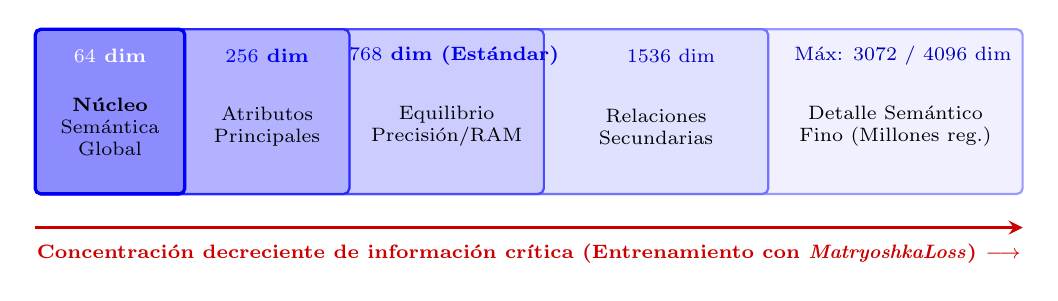
\begin{tikzpicture}[scale=0.95]
% Cajas anidadas Matryoshka
\draw[fill=blue!6, draw=blue!40, thick, rounded corners=2pt] (0,0) rectangle (13.2, 2.2);
\node[font=\scriptsize, blue!70!black] at (11.6, 1.85) {Máx: $3072$ / $4096$ dim};

\draw[fill=blue!12, draw=blue!55, thick, rounded corners=2pt] (0,0) rectangle (9.8, 2.2);
\node[font=\scriptsize, blue!80!black] at (8.5, 1.85) {$1536$ dim};

\draw[fill=blue!20, draw=blue!70, thick, rounded corners=2pt] (0,0) rectangle (6.8, 2.2);
\node[font=\scriptsize\bfseries, blue!90!black] at (5.6, 1.85) {$768$ dim (Estándar)};

\draw[fill=blue!30, draw=blue!85, thick, rounded corners=2pt] (0,0) rectangle (4.2, 2.2);
\node[font=\scriptsize\bfseries, blue!95!black] at (3.1, 1.85) {$256$ dim};

\draw[fill=blue!45, draw=blue!95!black, very thick, rounded corners=2pt] (0,0) rectangle (2.0, 2.2);
\node[font=\scriptsize\bfseries, white] at (1.0, 1.85) {$64$ dim};

% Etiquetas inferiores de densidad de información
\node[font=\scriptsize, align=center] at (1.0, 0.9) {\textbf{Núcleo}\\Semántica\\Global};
\node[font=\scriptsize, align=center] at (3.1, 0.9) {Atributos\\Principales};
\node[font=\scriptsize, align=center] at (5.5, 0.9) {Equilibrio\\Precisión/RAM};
\node[font=\scriptsize, align=center] at (8.3, 0.9) {Relaciones\\Secundarias};
\node[font=\scriptsize, align=center] at (11.5, 0.9) {Detalle Semántico\\Fino (Millones reg.)};

% Flecha de gradiente de importancia
\draw[-stealth, very thick, red!80!black] (0, -0.45) -- (13.2, -0.45);
\node[font=\scriptsize\bfseries, red!80!black] at (6.6, -0.8) {Concentración decreciente de información crítica (Entrenamiento con \textit{MatryoshkaLoss}) $\longrightarrow$};
\end{tikzpicture}
\caption{Estructura jerárquica de un vector entrenado mediante \textit{Matryoshka Representation Learning} (MRL): las primeras dimensiones concentran la mayor carga semántica, permitiendo truncar el vector de salida para reducir exponencialmente el consumo de memoria RAM y latencia con penalizaciones mínimas de precisión \cite{learnopencv_qwen3, gemini_emb2_docs}.}
\label{fig:matryoshka_mrl}
\end{figure}

Ahora bien, desde el punto de vista de la implementación algorítmica rigurosa, truncar un vector unitario $\mathbf{v} \in \mathbb{R}^{D}$ (donde $\|\mathbf{v}\|_2 = 1$) a sus primeras $d < D$ componentes ($\mathbf{v}_{1:d}$) hace que la suma de cuadrados de las coordenadas retenidas sea estrictamente menor que la unidad ($\sum_{j=1}^{d} v_j^2 < 1$). Dado que los vectores truncados (por ejemplo, al configurar $d = 768$ o $d = 1536$ en lugar de las $3072$ dimensiones completas en \textit{Gemini Embedding 2}) no vienen normalizados de fábrica tras el corte, resulta obligatorio aplicar una etapa explícita de \textbf{re-normalización mediante la norma euclídea $L_2$} según se define en la Ecuación~\eqref{eq:renormalizacion_l2_mrl} antes de insertarlos en la base de datos vectorial \cite{gemini_emb2_docs}:

\begin{equation}
\hat{\mathbf{v}}_{1:d} = \frac{\mathbf{v}_{1:d}}{\|\mathbf{v}_{1:d}\|_2} = \frac{(v_1, v_2, \dots, v_d)^\top}{\sqrt{\sum_{j=1}^{d} v_j^2}}
\label{eq:renormalizacion_l2_mrl}
\end{equation}

Esta operación proyecta de nuevo el sub-vector truncado sobre la superficie de la hipersfera unitaria de dimensión $d$, garantizando que las búsquedas posteriores por Similitud del Coseno en motores como Qdrant mantengan su consistencia matemática y velocidad de cómputo.

\subsubsection{Análisis del Compromiso entre Precisión Semántica y Coste de Almacenamiento}
\label{subsubsec:compromiso_precision_almacenamiento}

La elección de la dimensionalidad operativa del espacio latente introduce un compromiso directo (\textit{trade-off}) de arquitectura entre la granularidad de discriminación semántica y los costes de infraestructura \cite{gemini_emb2_docs, qwen3_vl_emb2026}. Como se sintetiza en el Cuadro~\ref{tab:compromiso_dimensiones}, trabajar con el espacio completo de \textbf{3.072 dimensiones} en \textit{Gemini Embedding 2} (o \textbf{4.096 dimensiones} en \textit{Qwen3-VL-Embedding-8B}) permite capturar un nivel de detalle semántico superior, lo cual resulta determinante cuando la base de datos acumula millones de registros multimodales y se requiere evitar falsos positivos ante consultas altamente específicas \cite{gemini_emb2_docs, qwen3_vl_emb2026}.

\begin{table}[htbp]
\centering
\small
\setlength{\tabcolsep}{4.5pt}
\caption{Comparativa técnica del impacto de la dimensionalidad vectorial y el soporte MRL sobre la precisión semántica y el coste de almacenamiento en bases de datos vectoriales \cite{gemini_emb2_docs, qwen3_vl_emb2026}.}
\label{tab:compromiso_dimensiones}
\begin{tabularx}{\linewidth}{>{\raggedright\arraybackslash}p{2.7cm} >{\raggedright\arraybackslash}p{3.3cm} >{\centering\arraybackslash}p{1.6cm} >{\centering\arraybackslash}p{1.7cm} >{\raggedright\arraybackslash}X}
\toprule
\textbf{Configuración} & \textbf{Modelos de Referencia} & \textbf{Peso (FP32)} & \textbf{Norm. $L_2$} & \textbf{Caso de Uso Óptimo} \\
\midrule
4.096 dim (Máx. Open) & Qwen3-VL-Embedding-8B & 16,0 KB & Nativa & Máxima resolución en servidor GPU local \\
3.072 dim (Máx. Cloud) & Gemini Embedding 2 & 12,0 KB & Nativa & \textit{Baseline} de máxima precisión y millones de reg. \\
2.048 dim (Intermedia) & Qwen3-VL-Embedding-2B & 8,0 KB & Nativa / MRL & Despliegue local equilibrado en VRAM \\
1.536 dim (MRL Medio) & Gemini Embedding 2 & 6,0 KB & Post-corte & Reducción del 50\% en RAM con alta fidelidad \\
768 dim (Estándar) & Gemini 2 / EmbeddingGemma 2 & 3,0 KB & Post-corte & Ahorro del 75\% en BD y consultas ultrarrápidas \\
64 - 256 dim (Ultraligero) & Qwen3-VL / EmbeddingGemma 2 & 0,25 - 1,0 KB & Post-corte & \textit{Edge computing}, dispositivos móviles y pre-filtrado \\
\bottomrule
\end{tabularx}
\end{table}

Por el contrario, operar sobre un estándar de \textbf{768 dimensiones} (que constituye el tope nativo de modelos ligeros modulares como \textit{EmbeddingGemma 2} (con posibilidad de truncado adicional a $256$ o $128$ dimensiones) y uno de los puntos de corte recomendados en \textit{Gemini Embedding 2}) reduce exactamente en un $75\%$ la huella de memoria de cada vector respecto a las $3.072$ dimensiones (pasando de $12,0\,\text{KB}$ a $3,0\,\text{KB}$ por fragmento en precisión simple de 32 bits). Esta compresión hace que la base de datos vectorial resultante sea significativamente más económica de alojar en memoria RAM y más rápida de consultar localmente, a cambio de asumir una ligera reducción en la granularidad semántica fina frente al vector completo de $3.072$ dimensiones.

\subsubsection{Aprendizaje Contrastivo (\textit{InfoNCE}) y el Fenómeno de la Brecha Modal (\textit{Modality Gap})}
\label{subsubsec:infonce_modality_gap}

Desde el punto de vista de la optimización neuronal, la alineación geométrica entre consultas textuales y fragmentos audiovisuales se entrena mediante funciones objetivo contrastivas simétricas basadas en la pérdida \textbf{\textit{InfoNCE}} (\textit{Noise-Contrastive Estimation}) \cite{vandenoord2018cpc, radford2021clip}. Dado un lote (\textit{mini-batch}) de $B$ pares emparejados $\{(\mathbf{q}_i, \mathbf{v}_i)\}_{i=1}^{B}$ proyectados sobre la hiperesfera unitaria $\mathbb{S}^{d-1}$, el entrenamiento maximiza la similitud de los pares positivos en la diagonal frente a los $B-1$ distractores negativos del lote, modulando la concentración de la distribución mediante un hiperparámetro de temperatura $\tau > 0$:

\begin{equation}
\mathcal{L}_{\text{InfoNCE}} = -\frac{1}{2B} \sum_{i=1}^{B} \left[
\log \frac{\exp\!\left(\text{sim}_{\cos}(\mathbf{q}_i, \mathbf{v}_i) / \tau\right)}{\sum_{j=1}^{B} \exp\!\left(\text{sim}_{\cos}(\mathbf{q}_i, \mathbf{v}_j) / \tau\right)} +
\log \frac{\exp\!\left(\text{sim}_{\cos}(\mathbf{v}_i, \mathbf{q}_i) / \tau\right)}{\sum_{j=1}^{B} \exp\!\left(\text{sim}_{\cos}(\mathbf{v}_i, \mathbf{q}_j) / \tau\right)}
\right]
\label{eq:infonce_loss}
\end{equation}

En la Ecuación~\eqref{eq:infonce_loss}, la temperatura $\tau$ controla la severidad con la que se penalizan los ejemplos negativos cercanos. Sin embargo, Liang et al. \cite{liang2022modalitygap} demostraron un fenómeno topológico inherente a los espacios contrastivos multimodales denominado \textbf{\textit{Modality Gap} (Brecha Modal)}: debido a que los codificadores de distinta modalidad nacen en regiones cónicas disjuntas de $\mathbb{S}^{d-1}$ tras la inicialización aleatoria, y a que la pérdida InfoNCE depende exclusivamente de las \textit{diferencias relativas} entre los pares positivos y negativos escaladas por $1/\tau$, la optimización converge preservando un desplazamiento vectorial sistemático entre el subespacio textual y el subespacio visual/audiovisual.

Esta propiedad explica rigurosamente un hallazgo empírico central observado en la literatura y en nuestros experimentos sobre \textit{Gemini Embedding 2} y \textit{Qwen3-VL-Embedding}: incluso cuando un par consulta-fragmento constituye un acierto semántico inequívoco de rango \#1, su similitud del coseno cruzada (\textit{cross-modal}) rara vez se aproxima a $1,0$, agrupándose de manera natural dentro de la banda $[0{,}28;\, 0{,}50]$ (mientras que pares intramodales texto-texto alcanzan valores mucho mayores). En consecuencia, el \textit{Modality Gap} invalida cualquier mecanismo de filtrado basado en umbrales fijos de coseno en la Etapa 1 y fundamenta la necesidad teórica de delegar la discriminación definitiva y el rechazo de falsos positivos a un verificador bimodal de Etapa 2.